\section{Introduction}

\begin{frame}
	\frametitle{Challenging Problem}
	
	\vspace{0.6cm}
	
	\begin{center}
		\begin{tikzpicture}
			\node at (5.05,0) [draw=red,ultra thick,inner sep=0pt]
			{
				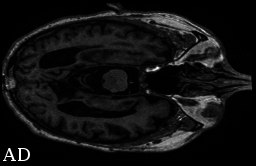
\includegraphics[scale=0.55]{Figures/AD}
			};
			\node at (0,0) [draw=red,ultra thick,inner sep=0pt]
			{
				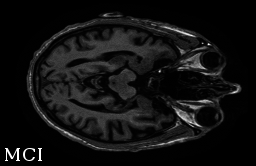
\includegraphics[scale=0.55]{Figures/MCI}
			};
			\node at (2.525,-3.3) [draw=red,ultra thick,inner sep=0pt]
			{
				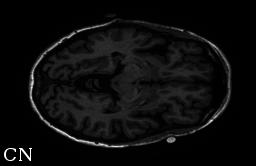
\includegraphics[scale=0.55]{Figures/CN}
			};
		\end{tikzpicture}
	\end{center}
\end{frame}

\begin{frame}
	\frametitle{Motivation}
	
	\Large
	
	\vspace{0.2cm}
	
	The cause of the Alzheimer's disease is still \textbf{poorly understood} and to date \textbf{no
	treatment} to stop or reverse its progression has been discovered.
	
	\vspace{0.5cm}
	
	In developed countries, the Alzheimer's disease is one of the most \textbf{financially costly}
	diseases due to \textbf{continuous treatments} as well as the \textbf{need} of assistance or
	supervision in daily activities.
\end{frame}

\begin{frame}
	\frametitle{Approach}
	\framesubtitle{Idea}
	
	\Large
	
	\vspace{0.2cm}
	
	The objective of this work is to present an \textbf{automated approach} for classifying the
	Alzheimer's disease from magnetic resonance imaging (MRI) patient brain scans.
	
	\vspace{0.1cm}
	
	The method is \textbf{fast} and \textbf{reliable} for a suitable and \textbf{straightforward
	deploy} in clinical applications by recognising the disease state of the patient.
	
	\vspace{-0.1cm}
	
	\begin{center}
		\begin{tikzpicture}
			\node at (-5.5,0) [draw=white,ultra thick,inner sep=0pt]
			{
				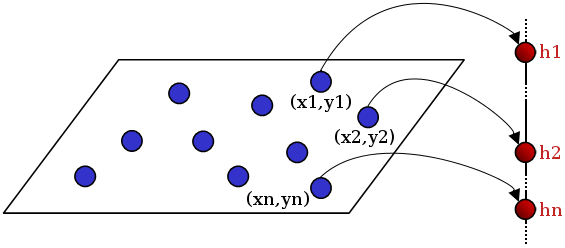
\includegraphics[scale=0.2]{Figures/CantorHash}
			};
			\node at (0,0) [draw=white,ultra thick,inner sep=0pt]
			{
				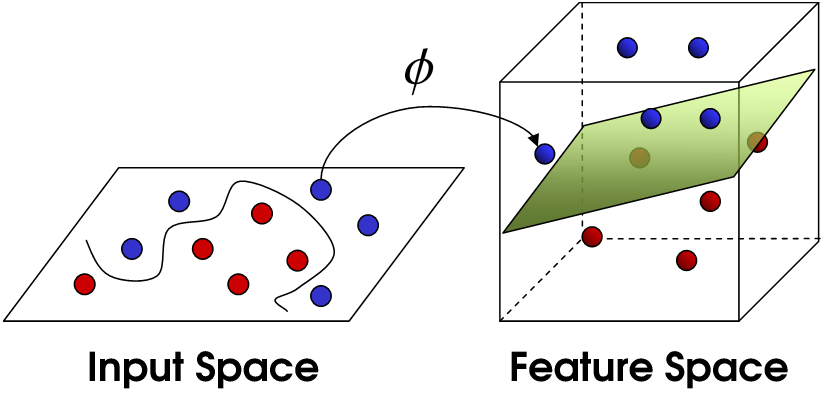
\includegraphics[scale=0.2]{Figures/SVM}
			};
		\end{tikzpicture}
	\end{center}
\end{frame}

\begin{frame}
	\frametitle{Approach}
	\framesubtitle{Results}
	
	\Large
	
	\vspace{0.2cm}
	
	We report the comparison on \textbf{two established} medical data sets (ADNI and OASIS).
	
	\vspace{0.5cm}
	
	In binary classification, our proposed approach \textbf{outperforms} most state-of-the-art
	techniques, while having comparable results with the others.
	
	\vspace{0.5cm}
	
	When dealing with three or four classes (i.e., all subjects) our method is the \textbf{only one}
	that reaches \textbf{remarkable} performance, outperforming state-of-the-art approaches.
\end{frame}
